\documentclass{standalone}
\usepackage{amsmath}
\usepackage{tikz}
\usetikzlibrary{arrows,shapes,positioning,shadows,trees}

\begin{document}
\begin{tikzpicture}
    \node (a) at (0,0) {
        \begin{tikzpicture}
            \filldraw[fill=gray!20,draw=white] (-2,0) -- (2,0) -- (2,1) -- (-2,1) -- (-2,0);
            \draw[-] (-2,0) -- (2,0);
        \node[fill,circle,inner sep=1pt,label=above right:$a$] at (1,1) {};
        \end{tikzpicture}
    };

    \node (b) at (8,0) {
        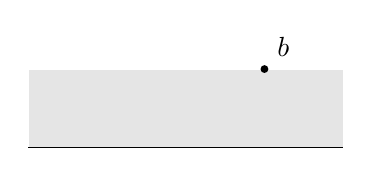
\begin{tikzpicture}
            \filldraw[fill=gray!20,draw=white] (-2,0) -- (2,0) -- (2,1) -- (-2,1) -- (-2,0);
            \draw[-] (-2,0) -- (2,0);
        \node[fill,circle,inner sep=1pt,label=above right:$b$] at (1,1) {};
        \end{tikzpicture}
    };

    \node (c) at (4,-4) {
        \begin{tikzpicture}
            \draw (0,0) circle (2);
            \node[fill,circle,inner sep=1pt,label=below:$O$] at (0,0) {};
        \end{tikzpicture}
    };

    \draw[->] (a) -- (c) node[midway,above right] {$f_1$};
    \draw[->] (b) -- (c) node[midway,below right] {$f_2$};
\end{tikzpicture}
\end{document}